\documentclass[crop,tikz]{standalone}
\usetikzlibrary{calc,patterns,decorations.pathmorphing,decorations.markings}
\usepackage{siunitx}
\begin{document}
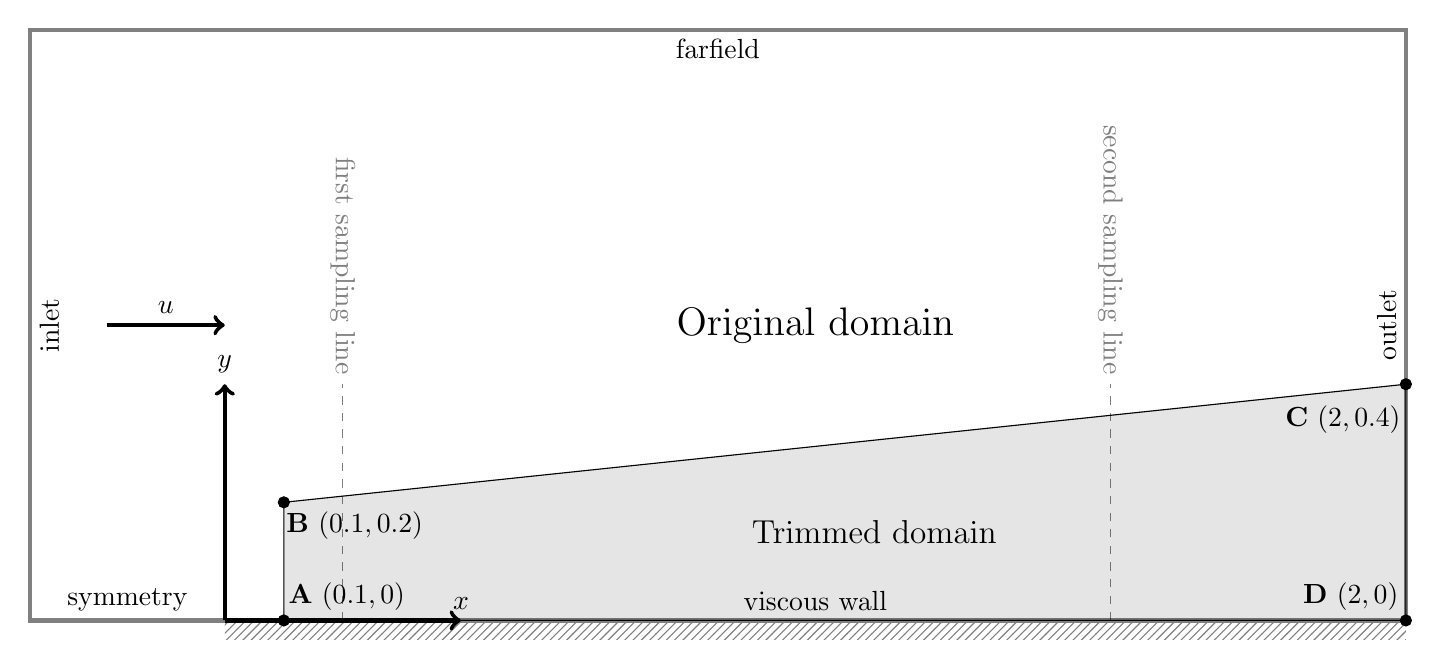
\begin{tikzpicture}
    \tikzstyle{ground}=[fill,pattern color=gray,pattern=north east lines,draw=none,minimum width=15cm,minimum height=0.2cm]
    \draw[scale=7.5,ultra thick, gray] (-0.33,0) -- (0,0) -- (2, 0) -- (2,1) -- (-0.33, 1) -- cycle;
    \draw (0,0) -- (15, 0) node [ground, midway, below] {};
    \node at (-0.33/2*7.5, 0) (symmetry) [above] {symmetry};
    \node at (1*7.5,0) (wall) [above] {viscous wall};
    \draw[gray] (2*7.5,1*7.5) -- (-0.33*7.5, 1*7.5) node [ midway, below, black] {farfield};
    \node at (-0.33*7.5, .5*7.5) (inlet) [rotate=90, below] {inlet};
    \node at (2*7.5, .5*7.5) (outlet) [rotate=90, above] {outlet};

    \draw[scale=7.5, dashed, opacity=0.5] (0.2, 0) -- (0.2, 0.4) node [above, left, rotate = -90] {first sampling line};
    \draw[scale=7.5, dashed, opacity=0.5] (1.5, 0) -- (1.5, 0.4) node [above, left, rotate = -90] {second sampling line};

    \draw[scale = 7.5, fill, opacity=0.1] (0.1, 0) -- (0.1,0.2) -- (2, 0.4) -- (2, 0) -- cycle;
    \draw[scale = 7.5] (0.1, 0) -- (0.1,0.2) -- (2, 0.4) -- (2, 0) -- cycle;
    
    \node at (0.1*7.5,0) (A) [xshift=0.8cm, yshift = 0.3cm] {\textbf{A} $(0.1, 0)$};
    \filldraw (0.1*7.5,0) circle (0.07);

    \node at (0.1*7.5,0.2*7.5) (B) [xshift=0.9cm, yshift = -0.3cm] {\textbf{B} $(0.1, 0.2)$};
    \filldraw (0.1*7.5,0.2*7.5) circle (0.07);

    \node at (2*7.5,0.4*7.5) (C) [xshift=-0.8cm, yshift=-0.45cm] {\textbf{C} $(2, 0.4)$};
    \filldraw (2*7.5,0.4*7.5) circle (0.07);

    \node at (2*7.5,0*7.5) (D) [xshift=-.7cm, above] {\textbf{D} $(2, 0)$};
    \filldraw (2*7.5,0*7.5) circle (0.07);

    \node at (1*7.5,0.5*7.5) (orDom) {\Large Original domain};
    \node at (1.1*7.5,0.15*7.5) (orDom) {\large Trimmed domain};

    \draw[ultra thick, ->, scale = 7.5] (-0.2,0.5) -- (0,0.5) node [midway, above] {$u$};

    \draw[->, ultra thick] (0,0) -- (3cm,0) node [above] {$x$};
    \draw[->, ultra thick] (0,0) -- (0,3) node [above] {$y$};

    

\end{tikzpicture}
\end{document}